\chapter{Conic Lab}
\label{sec:coniclab}
\section{Game Overview}
\label{sec:gameoverview}
Conic Lab is an innovative puzzle platformer game designed with the dual purpose of engaging players and educating them on the topic of conic sections, a fundamental area of precalculus. The game consists of two doors in which the left door is where the player spawns and the right door is where the player must go through. In this game, there are several obstacles or unpassable areas where players must use the different types of conic shapes in order to assist them in passing through those situations. The game aligns with the DepEd Learning Competencies for Precalculus, specifically targeting Learning Outcomes: (14) recognize the equation and important characteristics of the different types of conic sections, and (15) solve situational problems involving conic sections. The GBLE’s target users are SHS students that are currently taking lessons on Precalculus’ Analytical Geometry: Conic Sections, on which the game could help them further understand their lessons.

\section{Software Objectives}
\label{sec:softwareobjectives}
\subsection{General Objective}
\label{sec:genobjective}
The general objective of the Game-Based Learning Environment (GBLE) is to act as a support tool for player-learners to achieve the Learning Outcomes (LOs) in Precalculus Senior High School (SHS) and at the same time while keeping them engaged through interactive and immersive gameplay experiences.

\subsection{Specific Software Objectives}
\label{sec:specsoftwareobjectives}
The specific software objectives are as follows:
\begin{enumerate}
    \item To support player-learners in achieving the target Precalculus Learning Outcomes (LOs) through the game mechanics and elements of the Game-Based Learning Environment (GBLE) as Conic Lab integrates educational puzzles and interactive tutorials which are designed to reinforce the understanding and application of conic sections,
    \item To engage player-learners through the game’s visuals, mechanics, audio, and narrative, Conic Lab offers a cutesy art style with intuitive but fairly challenging gameplay.
\end{enumerate}

\section{Scope and Limitations}
\label{sec:gamescopelimitation}
The GBLE developed is meant to be used as a support tool only, meaning that the player-learners must already have previous knowledge regarding the LOs that the GBLE will cover. The game mechanics of the GBLE are based on the LOs of Precalculus, however, it will not cover the entire subject, but rather, selected LOs in the Analytical Geometry section, specifically conic sections. The LOs used as the basis of the GBLE were chosen based on the recommendations of a Precalculus expert, as well as previous related literature.
The narrative and characters of the GBLE are entirely fictional; any similarities to actual events or persons are purely coincidental. All resources such as visuals and audio found in the game will be taken from royalty free sources. Game mechanics from already developed games and the learning game principles will serve as the basis for the game mechanics of the GBLE.

\section{Architectural Design}
\label{sec:gamearchdesign}
The architectural design for the proposed GBLE will be composed of both learning and game mechanics. The game mechanics are meant to complement each learning mechanic to improve the learning experience of the players. The Foundation and Evaluation modules consist of the learning elements and which game mechanics would be created in order to integrate them into the game for the players to experience them.

\begin{figure}[H]
\hspace*{-1cm}
   \centering                  
   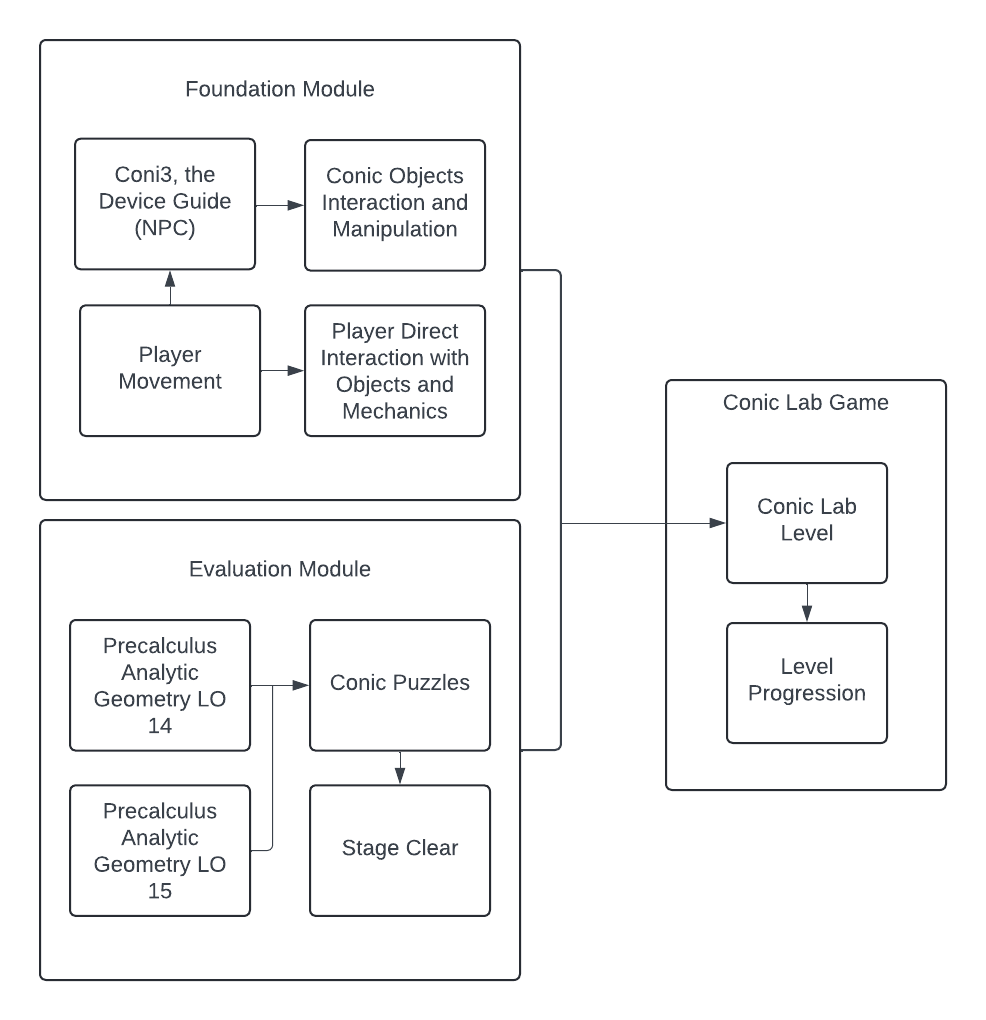
\includegraphics[width=400px,height=300px]{Chapter4/Architectural.png}      
   \caption{Architectural Design}
    \label{fig:Architectural}
\end{figure}

\subsection{Level Progression}
\label{sec:lvlprog}
Levels are divided into chapters in order to introduce each concept to the player-learner one by one. There will be a total of 4 chapters, one for each conic section: circle, ellipse, parabola, hyperbola, with 8-10 levels each to ensure the player-learner masters the concepts introduced in each chapter. Earlier levels within the chapter will be designed to be simple, only requiring minor alterations of the conic section (ex., only one variable can be altered). As the player-learner progresses to later levels in the chapter, puzzles will progressively increase in difficulty and require more alterations in the conic sections to complete the level.

\subsection{Coni3, Non-playable Character Guide and Device}
\label{sec:coni3}
The player-learner will be accompanied by a non-playable character (NPC) named Coni3 throughout the entire game. Coni3 will act as a guide and the main device with which the player-learner will interact. By interacting with the device, the respective values of H, K, A, and B can be altered to manipulate the shape of conic sections found in the level. A small guide can also be found, with the corresponding formulas and graphs for visualization for each conic section. In addition to this, Coni3 will assist player-learners when new mechanics are introduced through dialogue boxes.

\begin{figure}[H]
\hspace*{-1cm}
   \centering                  
   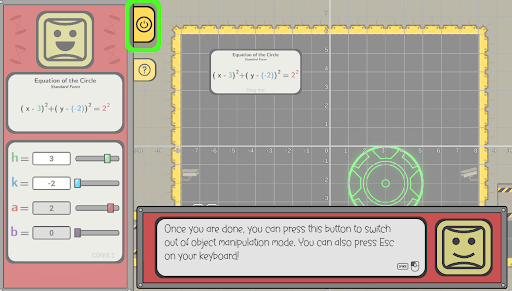
\includegraphics[width=300px,height=200px]{Chapter4/Coni3.png}      
   \caption{Meega Criteria for Game Quality Classification}
    \label{fig:MeegaCriteria}
\end{figure}

\subsection{Foundation Module}
\label{sec:foundationmodule}
This module aims to target one of the common challenges proposed by the Precalculus expert about why students were having difficulty learning Precalculus concepts. The tutorial guides the players on how to move the interactable objects and their character itself. This will help them go forward in several platform challenges within the game and they will be able to test their knowledge in conic sections through completing the game. 
These tutorials would include introducing the player to the required inputs for movement and demonstrating how to interact with game objects. New mechanics, such as linked objects, moving platforms, etc., will be introduced slowly as the player-learner progresses through the game with the assistance of the NPC guide.

\begin{figure}[H]
\hspace*{-1cm}
   \centering                  
   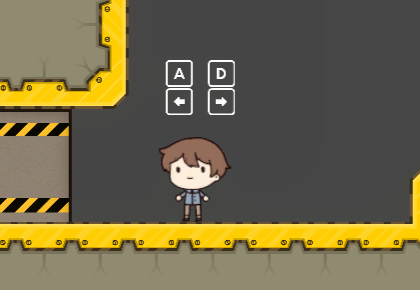
\includegraphics[width=300px,height=200px]{Chapter4/Foundation.png}      
   \caption{Player control tutorial}
    \label{fig:foundation}
\end{figure}

\subsection{Evaluation Module}
\label{sec:evaluationmodule}
For the evaluation module, there would be a series of puzzles that represent the different types of conic sections; these puzzles would be located around the level. The player is required to solve puzzles by transforming conic sections found in the level to traverse through the platforms, go through the exit gate, and complete the level. Different mechanics will be introduced throughout the game to make the levels more challenging and varied.

\begin{enumerate}
    \item \textbf{Conic Objects} - Objects resembling the conic sections are present throughout the entire game. The player learner can interact with and modify these objects using Coni3. These objects are represented by “Solid Light Constructs”, which are used as player obstructions or platforms.
\begin{figure}[H]
\hspace*{-1cm}
   \centering                  
   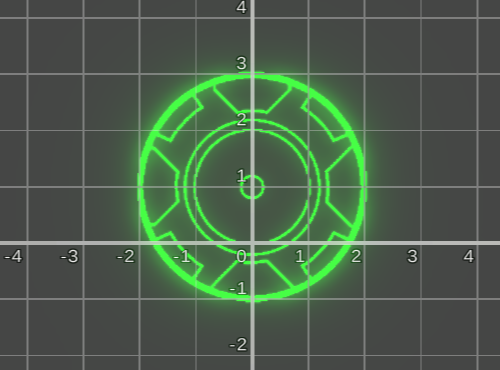
\includegraphics[width=300px,height=200px]{Chapter4/ConicObjects.png}      
   \caption{Sample of a Circle construct in the game}
    \label{fig:circleconstruct}
\end{figure}    
    \item \textbf{Key Shapes, Key Points, and Readers} - Just like Conic Objects, Key shapes may resemble one of the Conic Sections. Attached to these key shapes are key points; the key points represent the vertices (yellow) and the foci (blue) of a given conic section. The key points are then placed on to their color-matching readers. The readers act as a switch when a key point is properly placed onto it, triggering a different mechanism in the level and reversing the effect if the key point is removed.
\begin{figure}[H]
\hspace*{-1cm}
   \centering                  
   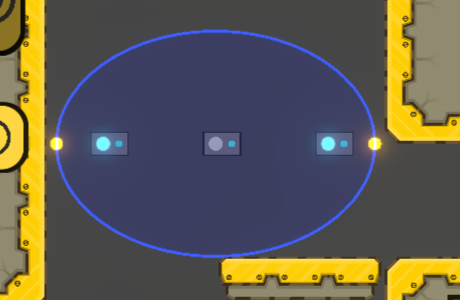
\includegraphics[width=300px,height=200px]{Chapter4/KeyShapes.png}      
   \caption{Keyshapes that requires the proper placement of foci of the ellipse }
    \label{fig:keyshapes}
\end{figure}
    \item \textbf{Pressure Plates} - Pressure plates will be activatable by the player-learner by placing weight on it, such can by placing an object on top of it or the player-learner stepping on it. Once activated, a different mechanism will be triggered at the level for the player-learner to progress (i.e., a gate opening). However, removing the weight on the pressure plate will reverse the effect it had.
\begin{figure}[H]
\hspace*{-1cm}
   \centering                  
   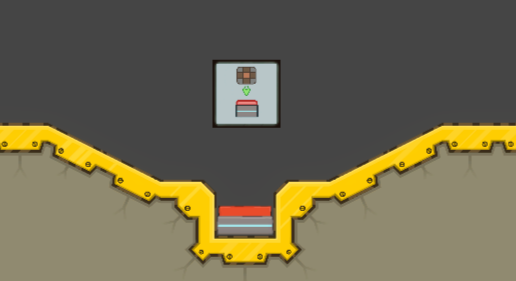
\includegraphics[width=300px,height=200px]{Chapter4/PressurePlates1.png}      
   \caption{Pressure plate with a helping instruction}
    \label{fig:pplates1}
\end{figure}
\begin{figure}[H]
\hspace*{-1cm}
   \centering                  
   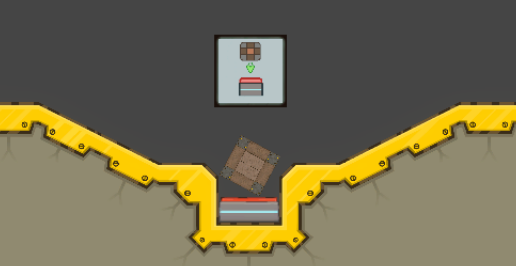
\includegraphics[width=300px,height=200px]{Chapter4/PressurePlates2.png}      
   \caption{Pressure plate being activated by applying weight to it}
    \label{fig:pplates2}
\end{figure}
    \item \textbf{Buttons} - Buttons are interactable by the player-learner and can be pressed by pressing the ‘E.’ on the keyboard. Once pressed, a different mechanism will be triggered in the level.
\begin{figure}[H]
\hspace*{-1cm}
   \centering                  
   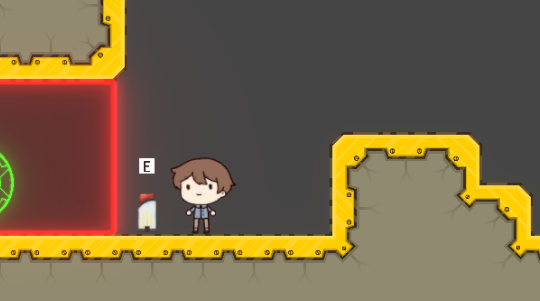
\includegraphics[width=300px,height=200px]{Chapter4/Buttons.png}      
   \caption{Players can interact with the buttons}
    \label{fig:buttons}
\end{figure}
    \item \textbf{Gates} - Gates are obstructions present within levels that the player-learner must open in order to get through.
\begin{figure}[H]
\hspace*{-1cm}
   \centering                  
   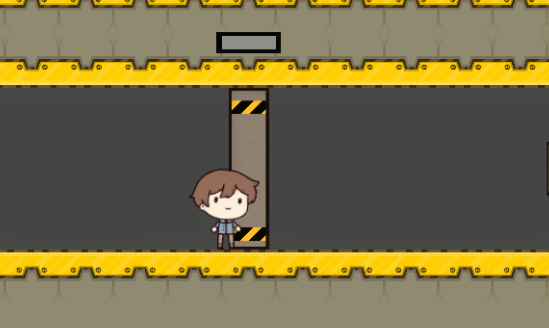
\includegraphics[width=300px,height=200px]{Chapter4/Gates.png}      
   \caption{}
    \label{fig:gates}
\end{figure}
    \item \textbf{Moving Platforms} - Moving platforms are platforms that will travel to designated points. A visual indicator will be present in order to differentiate which direction the platform will be going. The player-learner must interact with a different mechanic present within the level in order to activate the platforms.
\begin{figure}[H]
\hspace*{-1cm}
   \centering                  
   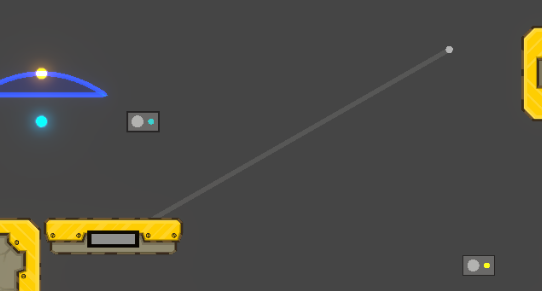
\includegraphics[width=300px,height=200px]{Chapter4/MovingPlatforms.png}      
   \caption{Moving platforms helps in crossing difficult gaps}
    \label{fig:keyshape}
\end{figure}
    \item \textbf{Disappearing Platforms} - Disappearing platforms are initially translucent, indicating that there is a possibility of making them visible. The player-learner must interact with a different mechanic present within the level in order to activate the platforms.
\begin{figure}[H]
\hspace*{-1cm}
   \centering                  
   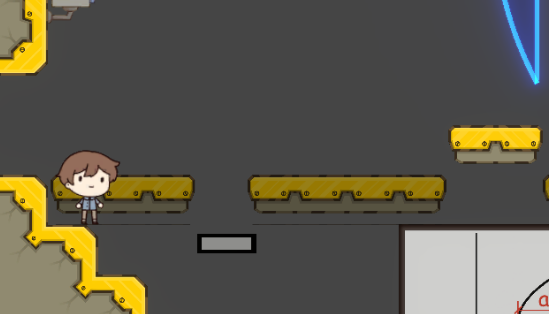
\includegraphics[width=300px,height=200px]{Chapter4/DisappearingPlatforms1.png}      
   \caption{An unactivated disappearing platform have a lighter shade than normal}
    \label{fig:dplatforms1}
\end{figure}
\begin{figure}[H]
\hspace*{-1cm}
   \centering                  
   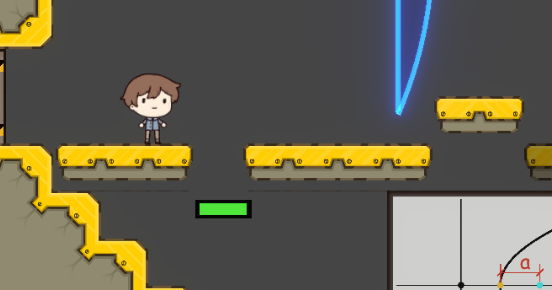
\includegraphics[width=300px,height=200px]{Chapter4/DisappearingPlatforms2.png}      
   \caption{When the proper mechanics get activated, it makes the platform appear}
    \label{fig:dplatforms2}
\end{figure}
    \item \textbf{Linked Objects} - Linked objects are objects that can be altered by the player-learner. The movement of one object causes the other object linked to it to move as well.
\begin{figure}[H]
\hspace*{-1cm}
   \centering                  
   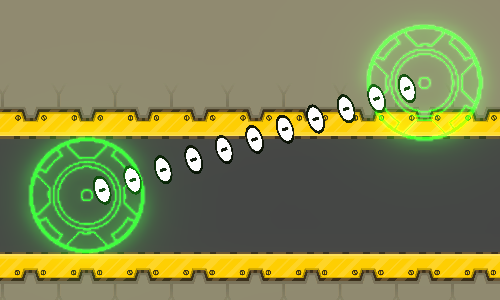
\includegraphics[width=300px,height=200px]{Chapter4/LinkedObjects.png}      
   \caption{A chain between constructs indicate that they are linked objects}
    \label{fig:linkedobjects}
\end{figure}
\end{enumerate}


\subsection{Software Functions}
The software functions of the GBLE are the following:

\begin{enumerate}
    \item \textbf{Main Menu} - The main menu is the screen that will be displayed to the player when the application is launched. Here, all the levels are displayed, and information on which levels have been completed is also contained.
    \item \textbf{Pause} - Inside each level, there will be a pause button in the upper right corner. Clicking on this opens a new interface with two possible selections: resume and level select.
    \item \textbf{Resume} - This is a button found when the pause button is clicked. Pressing this button simply returns the player back to the game screen.
    \item \textbf{Level Select} - This button is found when pressing the pause button. Clicking this button will return the player to the main menu.
    \item \textbf{Retry} - Similar to the pause button, the retry button is found on each level and is just beside the pause button in the upper right corner. This button simply restarts the level, moving the player back to the spawn point.
    \item \textbf{Device} - The device is found on the left side of the screen at each level. It is where the player is able to change the values of H,K, A, and b of each conic shape. 
    \item \textbf{Help} - This is the button found beside the device with a question mark symbol in it. Clicking on this allows the player to open a guide consisting of the formulas of each of the conic shapes and some other tips that could help deal with the different mechanics inside the game.
    \item \textbf{Back} - This is the button found beside the device above the help button with a power symbol. Pressing this button returns the player to the game screen.
    \item \textbf{Shape Interaction} - Clicking on a conic object “turns on” the device, allowing the player to manipulate the variables of the shape. When a conic object is clicked, the grid view is shown to the player, and the cartesian plane is overlaid onto the level to assist the players in determining where the shapes are located.
\end{enumerate}

\section{Physical Environment and Resources}
The GBLE was developed using Unity as its game engine, and was designed for desktop computers, and is able to be run even with a “low-end” PC. Inputs will only be accepted through the mouse and keyboard connected to the PC.


